% =============================================================================
%  XXI Simposio CEA de Control Inteligente (SCI 2026, Salamanca)
%  "Diseno industrial optimo con redes neuronales"
%  Plantilla oficial SCI 2023 (sciarticle + crc_SCI). Compilar con pdflatex.
% =============================================================================
\documentclass[5p,times,authoryear]{sciarticle}

\usepackage{crc_SCI}
\usepackage[spanish]{babel}
\usepackage[utf8]{inputenc}
\usepackage[T1]{fontenc}
\usepackage{amsmath}
\usepackage{amssymb}
\usepackage{bm}
\usepackage{booktabs}
\usepackage{graphicx}
\usepackage{epstopdf}
\usepackage{flushend}
\usepackage{float}
\usepackage{multicol}
\usepackage[most]{tcolorbox}
\usepackage{url}
\usepackage{lastpage}
\renewcommand{\lastpage}{\pageref{LastPage}}  % robust running-head page range
\graphicspath{{Figuras/}}

\addto\captionsspanish{\def\tablename{Tabla}}

% --- Running-head metadata required by crc_SCI ---
\volume{XXI}
\firstpage{1}
\journalname{Simposio CEA de Control Inteligente.}
\runauth{Scala y Lopez}

\begin{document}

\begin{frontmatter}

\dochead{XXI Simposio CEA de Control Inteligente}
\datesite{24--26 de junio de 2026, Salamanca, España}

\title{Diseño industrial óptimo con redes neuronales}

\author[A,B]{Scala, S.\corref{cor1}}
\author[A]{Lopez, R.\fnref{fn1}}

\cortext[cor1]{Autor para correspondencia.
\\
S. Scala: simone.scala@kuleuven.be, ORCID \url{https://orcid.org/0009-0005-6403-2815}
\\
Attribution-NonCommercial-ShareAlike 4.0 International (CC BY-NC-SA 4.0)
}
\fntext[fn1]{R. Lopez: robertolopez@artelnics.com, ORCID \url{https://orcid.org/0000-0003-3729-1465}}

\address[A]{Artelnics, C/ del Adaja 10, 37185 Villamayor, Salamanca, España.}
\address[B]{KU Leuven, Departamento de Ingeniería Química, Celestijnenlaan 200F, 3001 Lovaina, Bélgica.}

\begin{comocitar}
\begin{center}
\begin{tcolorbox}[frame hidden, width=\linewidth*2, colframe=white, colback=black!8!white]
\tocitearticle{Scala, S., Lopez, R. 2026. Optimal industrial design with neural networks. XXI Simposio CEA de Control Inteligente, Salamanca.}
\end{tcolorbox}
\end{center}
\end{comocitar}

\begin{abstract}
Presentamos un marco de optimización sin derivadas para hallar las
condiciones de operación óptimas de sistemas modelados mediante redes
neuronales entrenadas con datos. El método, denominado contracción
iterativa del dominio (IDC, \emph{iterative domain contraction}),
aprovecha el coste de evaluación casi nulo de la red para presupuestos de
muestreo inviables con simuladores físicos, y maneja de forma nativa
restricciones de caja, lineales y de fórmula, así como problemas
mono- y multiobjetivo. Implementado en la biblioteca de código abierto
OpenNN, se ilustra con dos casos. En el primero se minimiza la
fotodegradación de una mezcla fotovoltaica orgánica cuaternaria, sujeta a
una restricción de símplex y a una ventana funcional donante:aceptor,
obteniéndose una heterounión realista y físicamente utilizable. En el
segundo se aborda el diseño bi-objetivo de un casco de velero a velocidad
fija, donde la resistencia al avance y la manga del casco entran en
conflicto (un casco más ancho gana estabilidad y espacio interior pero
aumenta el arrastre); IDC traza un frente de Pareto denso que revela con
nitidez ese compromiso y su rodilla, sobre la que se sitúa el diseño
recomendado. En ambos casos los resultados son muy satisfactorios y
prometedores.
\end{abstract}

\begin{keyword}
Optimización basada en datos \sep Redes neuronales \sep Optimización sin
derivadas \sep Metodología de superficie de respuesta \sep Optimización
multiobjetivo \sep Manejo de restricciones.
\end{keyword}

\begin{englishtitle}
\noindent \textbf{Optimal industrial design with neural networks}
\end{englishtitle}

\begin{abstractIng}
We present a derivative-free framework for finding the optimal operating
conditions of systems modelled by data-trained neural networks. The
method, iterative domain contraction (IDC), exploits the near-zero
evaluation cost of the surrogate to afford sampling budgets infeasible
for physical simulators, and natively handles box, linear and formula
constraints as well as single- and multi-objective problems. Implemented
in the open-source library OpenNN, it is illustrated on two cases. The
first minimises the photodegradation of a quaternary organic photovoltaic
blend, subject to a simplex constraint and a functional donor:acceptor
window, yielding a realistic, physically usable heterojunction. The second
addresses the bi-objective design of a sailing-yacht hull at fixed speed,
where residuary resistance and hull beam conflict (a wider hull gains
stability and interior space but increases drag); IDC traces a dense
Pareto front that clearly reveals this trade-off and its knee, where the
recommended design lies. In both cases the results are very good and
promising.
\end{abstractIng}

\begin{keywordIng}
Data-driven optimization \sep Neural networks \sep Derivative-free
optimization \sep Response surface methodology \sep Multi-objective
optimization \sep Constraint handling.
\end{keywordIng}

\end{frontmatter}

\begin{multicols}{2}

% =============================================================================
\section{Introducción}
El \emph{diseño óptimo} de un proceso industrial consiste en fijar sus
variables controlables de modo que se minimice un coste, se maximice un
rendimiento o se satisfagan unas especificaciones. En muchos dominios
(tratamiento de aguas, metalurgia, procesos químicos, energía) la relación
entre esas variables y las respuestas medibles es demasiado compleja para
un modelado de primeros principios, pero se aproxima bien a partir de datos
observacionales. Una \emph{cadena de optimización basada en datos} consta
de tres etapas: (1)~recogida de datos del sistema físico,
(2)~entrenamiento de una red neuronal sustituta $f\colon\mathbb{R}^n\to
\mathbb{R}^m$ que asocia entradas y salidas, y (3)~optimización de las
entradas sobre la red entrenada para hallar la configuración óptima.

Las dos primeras etapas están bien cubiertas por el aprendizaje automático
moderno; la tercera, la \emph{optimización de la respuesta}, es el objeto de
este trabajo \citep{Myers2016,Derringer1980}. Enlaza además con el control
inteligente, pues las condiciones óptimas obtenidas no son sólo un diseño
estático, sino las \emph{consignas} (\emph{setpoints}) que la capa de
control debe alcanzar y mantener.

A diferencia de una superficie de respuesta polinómica, una red neuronal
captura no linealidades fuertes y su coste de evaluación es prácticamente
nulo ($10^4$--$10^6$ evaluaciones por segundo), lo que habilita presupuestos
de muestreo impensables con un simulador físico. Proponemos aprovechar esa
ventaja mediante la \emph{contracción iterativa del dominio} (IDC), que
comparte el esquema ``muestrear, seleccionar y contraer'' de la búsqueda
aleatoria acelerada \citep{Appel2003} pero está diseñada para el régimen de
muestreo masivo que permite el sustituto neuronal. El método está
implementado en la biblioteca de código abierto OpenNN \citep{OpenNN2026},
que también proporciona el entrenamiento de la red. Ilustramos la idea, sin
recargar el formalismo, sobre dos problemas industriales: uno mono-objetivo
con una restricción de símplex y otro bi-objetivo de diseño mecánico.

% =============================================================================
\section{Contracción iterativa del dominio}
\label{sec:metodo}
Sea $f$ una red neuronal entrenada con $p$ variables de entrada (continuas,
binarias o categóricas) y $q$ de salida. A cada variable se le puede
asignar una \emph{condición}: una restricción ($v\bowtie\beta$, con
$\bowtie\in\{=,\le,\ge,\in[l,u]\}$) o una designación como
\emph{objetivo} a minimizar o maximizar. Además se admiten
\emph{restricciones de fórmula} $g(\bm{x},\bm{y})\bowtie\beta$, afines o
no lineales, sobre entradas y/o salidas. El problema general es
\begin{equation}
  \max_{\bm{x}\in\mathcal{X}}\;\bigl(s_1\,o_1(\bm{x}),\ldots,s_k\,o_k(\bm{x})\bigr),
  \label{eq:problema}
\end{equation}
donde $o_j$ extrae el $j$-ésimo objetivo de la entrada o de la salida
$\bm{y}=f(\bm{x})$, $s_j=\pm1$ fija el sentido y $\mathcal{X}$ es el
conjunto factible. Con $k=1$ la solución es un punto óptimo; con
$k\ge 2$, el conjunto de Pareto.

El algoritmo (Figura~\ref{fig:diagramas}) parte de un dominio
hiperrectangular $\mathcal{D}^{(0)}$ derivado del rango de los datos de
entrenamiento y acotado por las condiciones. En cada iteración~$t$:
\begin{enumerate}\itemsep2pt
\item se generan $N$ entradas aleatorias en $\mathcal{D}^{(t)}$;
\item las restricciones \emph{afines de entrada} se reparan
  algebraicamente sobre la muestra (operador de reparación afín), de modo
  que cada punto satisface la restricción lineal sin rechazo;
\item se evalúa la red y se descartan los puntos que violan los límites
  de salida o las fórmulas;
\item los objetivos se normalizan a $[0,1]$ y se selecciona el
  subconjunto élite más cercano al \emph{punto utópico}
  $\hat{\bm{u}}^\ast=\bm{1}$ en distancia euclídea;
\item el dominio se contrae alrededor del mejor punto: para cada
  coordenada continua $h$,
  \begin{equation}
    l_h^{(t+1)}=\max\!\bigl(x_h^\ast-\tfrac{\gamma}{2}\Delta_h^{(t)},\,l_h^{(t)}\bigr),\;\;
    u_h^{(t+1)}=\min\!\bigl(x_h^\ast+\tfrac{\gamma}{2}\Delta_h^{(t)},\,u_h^{(t)}\bigr),
    \label{eq:reshape}
  \end{equation}
  con $\Delta_h^{(t)}=u_h^{(t)}-l_h^{(t)}$ y factor de zoom
  $\gamma\in(0,1)$.
\end{enumerate}
El bucle termina cuando el cambio relativo del objetivo cae por debajo de
una tolerancia o se agota el presupuesto de iteraciones. La reparación
afín garantiza factibilidad por construcción frente a restricciones
lineales, lo que ningún operador genético o de muestreo gaussiano asegura.
En el caso multiobjetivo (Figura~\ref{fig:diagramas_mo}) se mantiene un
frente de Pareto que se refina localmente en torno a los puntos no
dominados, monitorizado por dos métricas geométricas de calidad (hueco
interno y cercanía a la frontera).

\begin{figure*}[t]
\centering
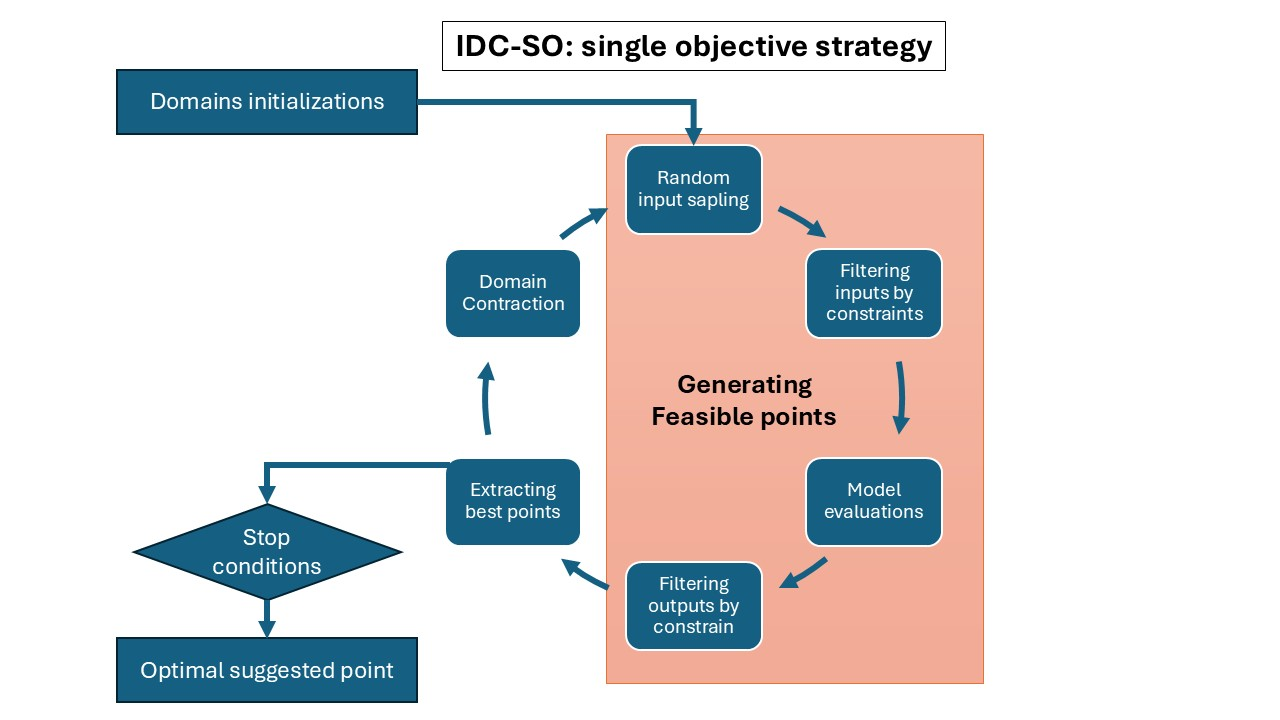
\includegraphics[width=0.86\textwidth]{fig_idc_so.jpg}
\caption{Estrategia mono-objetivo de IDC (IDC-SO): a partir del dominio
inicial, el lazo genera puntos factibles (muestreo aleatorio, filtrado de
entradas y salidas por restricciones, evaluación del modelo), extrae los
mejores y contrae el dominio hasta cumplir el criterio de parada.}
\label{fig:diagramas}
\end{figure*}

\begin{figure*}[t]
\centering
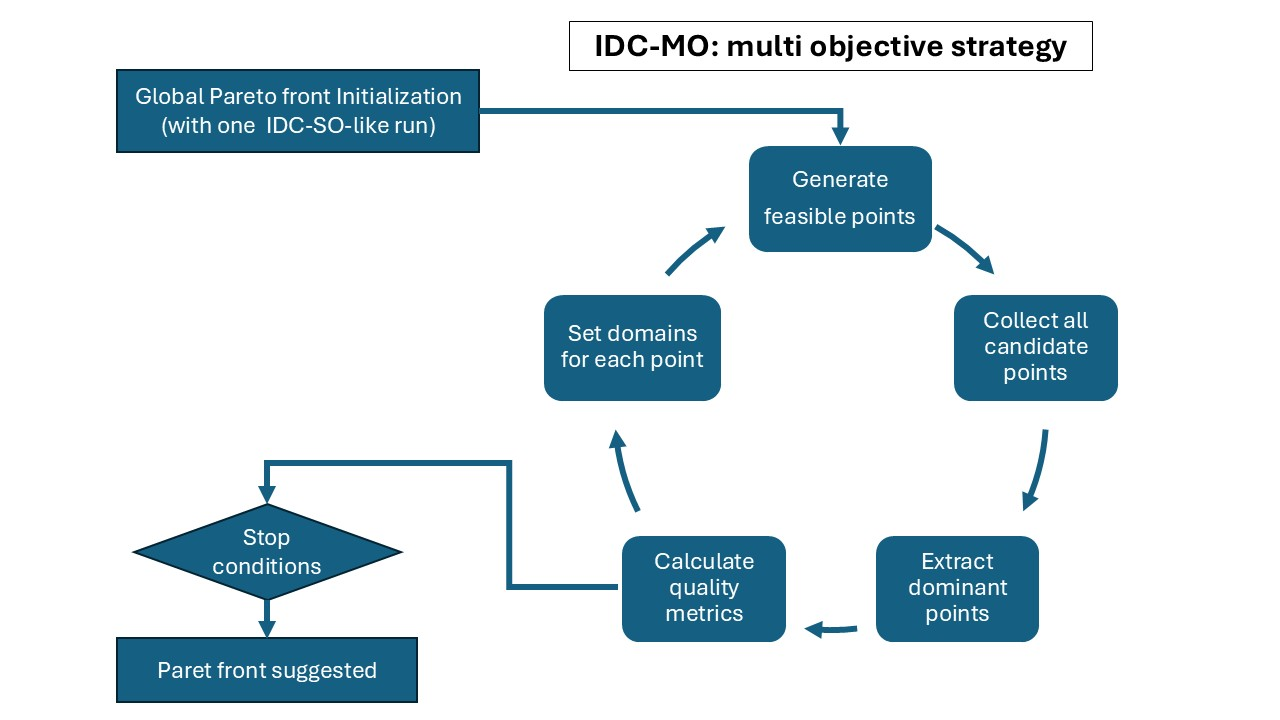
\includegraphics[width=0.86\textwidth]{fig_idc_mo.jpg}
\caption{Estrategia multiobjetivo de IDC (IDC-MO): se inicializa el frente
de Pareto global (una corrida tipo IDC-SO) y, para cada punto del frente,
se generan puntos factibles, se recopilan los candidatos, se extraen los
dominantes y se calculan métricas de calidad hasta la parada.}
\label{fig:diagramas_mo}
\end{figure*}

% =============================================================================
\section{Caso mono-objetivo: fotodegradación de una mezcla OPV}
\label{sec:so}
\paragraph{Problema físico} Las células solares orgánicas de heterounión en
volumen se fabrican mezclando dos donantes y dos aceptores; la fracción de
cada componente determina la morfología de la película y, con ella, su
estabilidad bajo iluminación. El problema está en que estas mezclas se
degradan con la luz, lo que acorta la vida útil del panel; hallar la
composición más fotoestable es por ello decisivo para la viabilidad
comercial de esta tecnología. Se usa el conjunto \texttt{photo\_wf3} de la
\emph{suite} Olympus \citep{Hase2021}, con $1040$ mezclas cuaternarias
medidas: dos donantes (WF3, el polímero de banda ancha PBQ-QF, y P3HT) y
dos aceptores (PCBM, fullereno, y oIDTBR, no fullereno) \citep{Langner2020}.

\paragraph{Formalización y modelo} Las cuatro fracciones másicas
$\bm{x}=(x_1,x_2,x_3,x_4)$ deben minimizar la fotodegradación medida
$y(\bm{x})$ sujetas, primero, al \emph{símplex}
\begin{equation}
  x_1+x_2+x_3+x_4=1,\qquad x_i\ge 0,
  \label{eq:simplex}
\end{equation}
una igualdad afín que reduce el espacio factible a un volumen de medida
nula dentro del cubo $[0,1]^4$. Ahora bien, minimizar sólo la
fotoestabilidad degenera: como el donante es la principal vía de
degradación, el óptimo tiende a una mezcla \emph{sin donante}, que no es una
célula solar. Un dispositivo de heterounión necesita sendas redes
percolantes de donante y de aceptor y, en operación, cada fotón absorbido
transfiere \emph{un} electrón del donante al aceptor en la interfaz, de modo
que el balance estequiométrico de carga es $\approx\!1{:}1$. Imponemos por
ello una \emph{ventana funcional donante:aceptor} sobre la fracción total de
donante (WF3${}+{}$P3HT):
\begin{equation}
  0{,}4 \le x_1+x_2 \le 0{,}6,
  \label{eq:da}
\end{equation}
esto es, una relación donante:aceptor entre $2{:}3$ y $3{:}2$. La campaña
original \citep{Langner2020} sólo imponía el símplex; esta ventana es una
elección de modelado nuestra para garantizar un dispositivo realista, y
constituye una restricción lineal adicional que IDC maneja de forma nativa
junto al símplex. Como sustituto $y(\bm{x})$ se entrena con OpenNN una red
con una capa oculta de $8$ neuronas, que alcanza $R^2=0{,}77$ sobre los
$1040$ datos (Figura~\ref{fig:gof_photo}); el interés del caso reside sobre
todo en el manejo simultáneo de las dos restricciones lineales.

\begin{figure}[H]
\centering
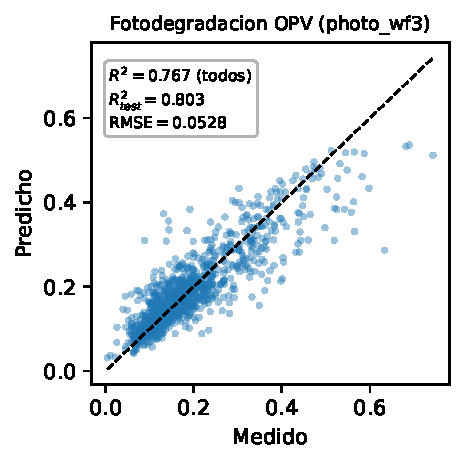
\includegraphics[width=5.2cm]{fig_gof_photo_wf3.pdf}
\caption{Bondad de ajuste del sustituto de OpenNN ($8$ neuronas) para la
fotodegradación de la mezcla OPV: $R^2=0{,}77$ sobre las $1040$ mezclas
($R^2=0{,}80$ en el conjunto de test).}
\label{fig:gof_photo}
\end{figure}

\paragraph{Diseño óptimo} Ejecutamos IDC sobre la red entrenada con los
$1040$ datos, con un presupuesto de $40\,000$ evaluaciones. Gracias al
operador de reparación afín, el punto devuelto satisface a la vez el símplex
y la ventana donante:aceptor (\emph{factibilidad por construcción}). La
mezcla óptima hallada
(Tabla~\ref{tab:so}) es una heterounión realista (donante WF3
$\approx\!0{,}41$ y aceptor fullereno PCBM $\approx\!0{,}59$, relación
donante:aceptor $\approx\!1{:}1{,}4$) con una fotodegradación de $0{,}056$ y
el 100\,\% de factibilidad. El coste de exigir un dispositivo funcional es
modesto: la degradación sólo sube de $\approx\!0{,}03$ (óptimo degenerado
sin donante) a $0{,}056$, a cambio de una solución físicamente utilizable.

\begin{table}[H]
\centering
\caption{Caso \texttt{photo\_wf3}: diseño óptimo hallado por IDC.}
\label{tab:so}
\begin{tabular}{l c}
\hline
Variable & Valor óptimo \\
\hline
WF3 (donante) & 0.409 \\
P3HT (donante) & 0.000 \\
PCBM (aceptor) & 0.591 \\
oIDTBR (aceptor) & 0.000 \\
\hline
Donante total / aceptor total & 0.41 / 0.59 \\
Relación donante:aceptor & $1:1.44$ \\
Fotodegradación & 0.0557 \\
Factibilidad (símplex + D:A) & 100\,\% \\
\hline
\end{tabular}
\end{table}

% =============================================================================
\section{Caso multiobjetivo: diseño de un casco de velero}
\label{sec:mo}
\paragraph{Problema físico} El conjunto \emph{Yacht Hydrodynamics} (serie
sistemática de Delft) relaciona cinco coeficientes geométricos del casco y
el número de Froude (velocidad) con la resistencia residual por unidad de
peso \citep{OrtigosaLopez2007}, el mismo problema con el que se gestó
OpenNN. El problema de diseño reside en un conflicto entre objetivos: a una
velocidad de crucero fija, un casco más ancho (menor relación eslora/manga)
ofrece más estabilidad y espacio de cubierta y bodega, pero a costa de una
mayor resistencia y, por tanto, de un mayor consumo. Acertar con ese
equilibrio es una decisión central del diseño naval.

\paragraph{Formalización y modelo} A partir de $308$ medidas reales de canal
de ensayos, y fijando el número de Froude a la \emph{media del conjunto}
($0{,}2875$) como restricción de igualdad, se busca \emph{minimizar la
resistencia residual} (salida de la red) y \emph{maximizar la manga}, esto
es, minimizar la relación eslora/manga $L/B$ (una entrada), con los cuatro
coeficientes restantes del casco libres dentro del envolvente de Delft; en
el sustituto, $L/B$ y la resistencia correlacionan negativamente
($-0{,}61$). El selector \emph{growing neurons} de OpenNN encuentra una red
compacta de $4$ neuronas que alcanza $R^2=0{,}995$ sobre todo el conjunto y
$R^2=0{,}99$ en el de test (Figura~\ref{fig:gof}), confirmando que una
arquitectura pequeña y bien dimensionada generaliza sin dificultad.

\begin{figure}[H]
\centering
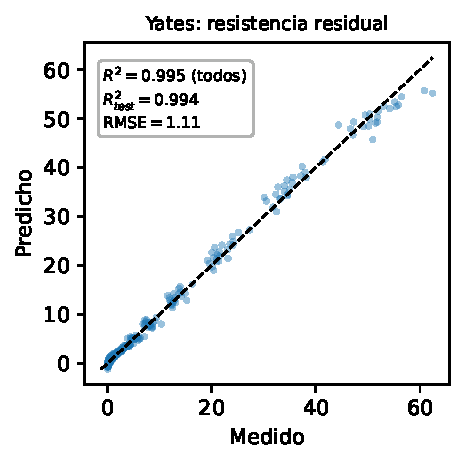
\includegraphics[width=5.2cm]{fig_gof_yacht.pdf}
\caption{Bondad de ajuste del sustituto de OpenNN para la resistencia
residual del velero ($4$ neuronas): $R^2=0{,}995$ sobre las $308$ medidas
($R^2=0{,}99$ en el conjunto de test).}
\label{fig:gof}
\end{figure}

\paragraph{Diseño óptimo} Ejecutamos IDC con un presupuesto de $40\,000$
evaluaciones. El muestreo masivo dirigido al punto utópico puebla
densamente el frente con unos $270$ cascos no dominados
(Tabla~\ref{tab:mo}). Normalizamos cada objetivo respecto a su propio rango
sobre el frente, de modo que éste recorre la caja unidad de esquina a
esquina; el área bajo la curva es el hipervolumen normalizado, $0{,}59$
(Figura~\ref{fig:pareto}). Normalizar en cambio respecto al rango del
conjunto de datos completo elevaría el hipervolumen a $\approx0{,}98$, pero
comprimiría el frente en una franja estrecha y ocultaría la forma del
compromiso. Éste es claro: al ensanchar el casco (reducir $L/B$ de $3{,}64$
a $2{,}73$) la resistencia residual mínima sube de $\approx0{,}5$ a
$\approx2{,}3$, con una rodilla bien definida en la región central. El
\emph{punto recomendado}, el más cercano al punto utópico (punto azul en la
Figura~\ref{fig:pareto}, Tabla~\ref{tab:mo}), cae precisamente en esa
rodilla: un casco de manga intermedia ($L/B\approx3{,}06$) con una
resistencia residual de $\approx1{,}4$, que equilibra ambos objetivos.

\begin{figure}[H]
\centering
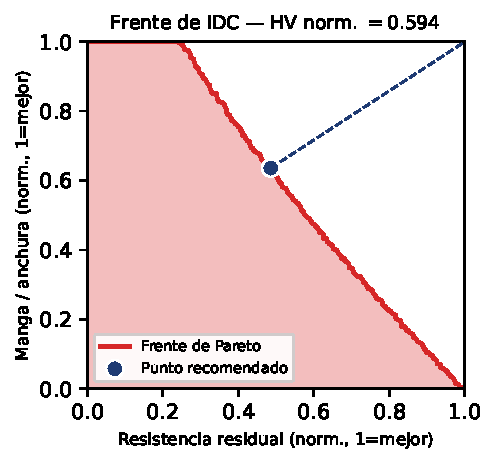
\includegraphics[width=5.6cm]{fig_normhv_yacht.pdf}
\caption{Frente de Pareto de IDC (resistencia frente a manga, esto es la
relación eslora/manga $L/B$, a Froude fijo). Cada eje se normaliza respecto
al propio rango del frente ($1=$ mejor); el área sombreada es el
hipervolumen normalizado ($=0{,}59$). Se aprecian el compromiso entre ambos
objetivos y la rodilla en la que se sitúa el punto recomendado (azul), unido
al punto utópico.}
\label{fig:pareto}
\end{figure}

\begin{table}[H]
\centering
\caption{Resultado de IDC en el caso \emph{yacht} bi-objetivo:
$|\mathcal{P}|$ (tamaño del frente), HV normalizado en $[0,1]$ ($1=$ ideal)
y el punto recomendado (más cercano al utópico).}
\label{tab:mo}
\begin{tabular}{l c}
\hline
Métrica & Valor \\
\hline
HV normalizado & 0.594 \\
Tamaño del frente $|\mathcal{P}|$ & 272 \\
\hline
\multicolumn{2}{l}{\emph{Punto recomendado (más cercano al utópico)}}\\
\quad Resistencia residual & 1.389 \\
\quad Relación eslora/manga $L/B$ & 3.060 \\
\hline
\end{tabular}
\end{table}

% =============================================================================
\section{Conclusiones}
La contracción iterativa del dominio cierra la cadena dato $\to$ red
$\to$ optimización con un algoritmo simple, pocos hiperparámetros y
manejo nativo de variables mixtas y restricciones. Su reparación afín
garantiza factibilidad por construcción frente a restricciones lineales
(decisiva en el caso del símplex) y su muestreo masivo, habilitado por el
coste casi nulo del sustituto, produce frentes de Pareto densos.
Como trabajo en curso se extiende la validación a problemas industriales
de mayor escala, en particular al tratamiento de aguas residuales, con
objetivos de coste frente a calidad del efluente. El código
y los datos de reproducción están disponibles en
\url{https://github.com/Siscanalysis/IDC}, y la biblioteca OpenNN en
\url{https://github.com/Artelnics/opennn}.

% =============================================================================
\section*{Agradecimientos}
Funded by the European Union (Marie Sk\l{}odowska-Curie Grant Agreement
no.\ 101169541, NEUTEN). Views and opinions expressed are however
those of the author(s) only and do not necessarily reflect those of the
European Union or the European Research Executive Agency (REA). Neither
the European Union nor the granting authority can be held responsible for
them.

\bibliographystyle{elsarticle-harv}
\bibliography{referencias}

\end{multicols}
\end{document}
